%% Bachelor Thesis Template of Xidian Uniersity
%%   for using XDBAthesis package with LaTeX
%%
%% Created by Xue-Jilong(xuejilong@gmail.com)
%%
%% template.tex v0.1, 2011/03/21


\documentclass[xetex,adobefonts,master]{XDBAthesis}
% 选项说明:
% dvipdfm  使用 dvipdfm(x) 生成最终的 PDF 文档 (缺省设置)
% dvips    使用 dvips 生成最终的 PS 文档
% pdftex   使用 pdfLaTeX 生成最终的 PDF 文档
% xetex    使用 XeLaTeX 生成 PD F文档
% adobefonts 使用 Adobe 中文字体
% winfonts 使用 Windows 中文字体
% master   用于生成硕士学位论文

% 图形文件的搜索路径
\graphicspath{{chapter-utf8/}{figures/}}

\begin{document}
%%----------------- 封面部分 ----------------- %%
    \schoolnumber{07071050}
    \title{复杂网络的数学模型研究与应用}{}   %%题目超过14个字把剩下的放到第二个空
    \entitle{Research and Application of}{ Mathematic Model of Complex Network}   %%题目超过14个字把剩下的放到第二个空
    \major{数学与应用数学}
    \author{薛继龙}
    \advisor{齐小刚}
    \date{二〇一二年一月}
    \majorclass{理科}

    \identifier{007}
    \classnumber{1-1(分类号)}
    \classification{公开}
    \maketitle

%%----------------- 前言部分 ----------------- %%
    \frontmatter
    \pagestyle{empty}
    \begin{center}
\heiti\zihao{3}西安电子科技大学\\[5mm]
	学位论文独创性(或创新性)声明
\end{center}\vspace{1cm}

\songti\zihao{-4}秉承学校严谨的学分和优良的科学道德,本人声明所呈交的论文是我个人
在导师指导下进行的研究工作及取得的研究成果。尽我所知,除了文中特别加以标注
和致谢中所罗列的内容以外,论文中不包含其他人已经发表或撰写过的研究成果;
也不包含为获得西安电子科技大学或其它教育机构的学位或证书而使用过的材
料。与我一同工作的同志对本研究所做的任何贡献均已在论文中做了明确的说明
并表示了谢意。

申请学位论文与资料若有不实之处,本人承担一切相关的法律责任。\\[3mm]

	本人签名:\rule{2.6cm}{0.75pt}  \hspace{3cm}  日期\rule{3cm}{0.75pt}\\[2cm]
	
\begin{center}
\heiti\zihao{3}西安电子科技大学\\[5mm]
	关于论文使用授权的说明
\end{center}\vspace{1cm}

\songti\zihao{-4}本人完全了解西安电子科技大学有关保留和使用学位论文的规定,即:研究
生在校攻读学位期间论文工作的知识产权单位属西安电子科技大学。学校有权保
留送交论文的复印件,允许查阅和借阅论文;学校可以公布论文的全部或部分内
容,可以允许采用影印、缩印或其它复制手段保存论文。同时本人保证,毕业后
结合学位论文研究课题再撰写的文章一律署名单位为西安电子科技大学。(保密的
论文在解密后遵守此规定)

本学位论文属于保密,在\rule{6mm}{0.75pt}年解密后适用本授权书。\\[3mm]

	本人签名:\rule{2.6cm}{0.75pt}  \hspace{3cm}  日期\rule{3cm}{0.75pt}\\[3mm]

	导师签名:\rule{2.6cm}{0.75pt}  \hspace{3cm}  日期\rule{3cm}{0.75pt}           

    
\begin{abstract}
本文介绍了西电版的\LaTeX{}~本科毕业设计论文模板,该模板是基于\CTeX{}~中
文宏包开发,指在为西安电子科技大学的本科毕业生提供一个简单、专业、有效的
排版工具,且该版本不打算加入研究生毕业论文和博士生毕业论文,因为定制模板
也是一个很复杂的事情,如果有可能的话,后期可能继续单独写研究生和博士生的
\LaTeX{}~模板。作者本着为西电同学服务的原则开发,并不承担一切有关责任与
义务,如维护、更新等,但欢迎提交~\texttt{BUG}~。祝西安电子科技大学的同学前程似锦。

西安电子科技大学是以信息与电子学科为主,工、理、管、
文多学科协调发展的全国重点大学,直属教育部,是国家“211工程”立项建设的重
点高校之一,是全国56所设有研究生院的高校之一,37所示范性软件学院的高校之一,
也是全国20所获批设立集成电路人才培养基地的高校之一。

1931年诞生于江西瑞金的中央军委无线电学校,是毛泽东等老一辈革命家亲手创建的第一所工程技
术学校。1958年学校迁址西安,1966年转为地方建制,1988年定为现名。建校79年来,
学校始终得到了党和国家的高度重视,是我国“一五”重点建设的项目之一,也是1959
年中央首批批准的全国20所重点大学之一。20世纪60年代,学校就以“西军电”之称
蜚声海内外。毛泽东同志曾先后两次为学校题词:“全心全意为人民服务”、“艰苦朴素”。
学校现建设有南北两个校区,总占地面积4000亩,校舍建筑面积130多万平方米,
图书馆藏书近420万册。

校现有各类在校生3万余人,其中博士研究生1700余人,
硕士研究生8100余人,设有通信工程学院、电子工程学院、计算机学院、机电工程学院、
技术物理学院、经济管理学院、理学院、人文学院、示范性软件学院、微电子学院、国际教育学院、
生命科学技术学院、网络与继续教育学院以及长安学院等14个学院。

\keywords{西电,论文,毕业设计,模板}
\end{abstract}

\begin{englishabstract}
This page is English abstract test.English is a West Germanic language
that arose in the Anglo-Saxon kingdoms of England and spread into what
was to become south-east Scotland under the influence of the Anglian medieval
kingdom of Northumbria. Following the economic, political, military, scientific,
cultural, and colonial influence of Great Britain and the United Kingdom from
the 18th century, via the British Empire, and of the United States since the
mid-20th century, it has been widely dispersed around the world, become the
leading language of international discourse, and has acquired use as lingua
franca in many regions. It is widely learned as a second language and used
as an official language of the European Union and many Commonwealth countries.

This page is English abstract test.English is a West Germanic language
that arose in the Anglo-Saxon kingdoms of England and spread into what
was to become south-east Scotland under the influence of the Anglian medieval
kingdom of Northumbria. Following the economic, political, military, scientific,
cultural, and colonial influence of Great Britain and the United Kingdom from
the 18th century, via the British Empire, and of the United States since the
mid-20th century, it has been widely dispersed around the world, become the
leading language of international discourse, and has acquired use as lingua
franca in many regions. It is widely learned as a second language and used
as an official language of the European Union and many Commonwealth countries.

This page is English abstract test.English is a West Germanic language
that arose in the Anglo-Saxon kingdoms of England and spread into what
was to become south-east Scotland under the influence of the Anglian medieval
kingdom of Northumbria.

\englishkeywords{Xidian, University, Thesis, Template}
\end{englishabstract}


    \tableofcontents

%%----------------- 正文部分 ----------------- %%
    \mainmatter
    \pagestyle{content}
    
\chapter{引言}
\label{chap:introduction}

本文介绍了西电版的\LaTeX{}~本科毕业设计论文模板,该模板是基于\CTeX{}~中
文宏包开发,指在为西安电子科技大学的本科毕业生提供一个简单、专业、有效的
排版工具,且该版本不打算加入研究生毕业论文和博士生毕业论文,因为定制模板
也是一个很复杂的事情,如果有可能的话,后期可能继续单独写研究生和博士生的
\LaTeX{}~模板。作者本着为西电同学服务的原则开发,并不承担一切有关责任与
义务,如维护、更新等,但欢迎提交~\texttt{BUG}~。祝西安电子科技大学的同学前程似锦。

本模板严格按照西安电子科技大学教务处教学实践中心下发的最新2010本科生毕业设计
论文要求设计制作,经过初步测试,已经完全符合要求,但是这不能保证完全无误,所
以望同学们使用时仔细慎重,如一经发现任何不符合要求之处,请联系\href{mailto:xuejilong@gmail.com}{xuejilong@gmail.com}
~进行修改,本项目的主页是\href{code.google.com/p/xdba-thesis}{code.google.com/p/xdba-thesis}~,欢迎下载最新
 版本。

\LaTeX{}~是一种高质量的排版工具,编写宏包目的是简化学位论文的撰写,使得论文
作者可以将精力集中到论文的内容上而不是浪费在版面设置上。同时宏包在符合学位
论文撰写要求的基础上尽可能地进行美化,其中还参考了出版界的一些排版规范。所以
极力推介大家使用。

\section{系统环境}
由于本模板未在其它任何环境下试用,所以提供开发环境,以便正常使用。该宏包是基于
最新的\CTeX v2.9.0.152~ 中文套装\cite{site:ctex}环境下开发编写,底层支持~CCT~和~CJK~两种中文~\LaTeX{}~
系统。所以可以在该环境在正常使用和二次修改。

按常规,该包宏包可以在目前大多数的~\TeX{}~系统中使用,例如~C\TeX{}、~MiK\TeX{}、
~te\TeX{}、~fp\TeX{}。

此外,~\texttt{XDBAthesis}~宏包还使用了宏包~amsmath、~amsthm、~amsfonts、
~amssymb、~bm~、~hyperref~和~caption2~。目前大多数的~\TeX{}~系统中都包含有这些宏包。
中包含了以上列出的各种宏包,用户无需额外的设置即可使用。

\section{完善与更新}

XDBAthesis宏包的最新版本可以从~\url{http://code.google.com/p/xdba-thesis}~网站下载。
该宏包包含两个文件:~\texttt{XDBAthesis.cls}~和~\texttt{XDBAthesis.cfg}。
简单方便的安装方法是将宏包文件和学位论文~\texttt{.tex}~文件放置在同一目录下。

同时,宏包还提供了一个使用模板,也就是这份说明文档的源文件。用户可以通过修改
这个模板来编写自己的学位论文。

由于该包首次制作,难免有问题,所以有使用发现的,其及时与作者联系,或者到上述网站参与
维护更新。


\section{宏包定制}

\texttt{XDBAthesis}~宏包的设置都保存在~\texttt{XDBAthesis.cfg}~文件中。
用户可以在~\texttt{.tex}~中通过宏包提供的命令修改设置。对于常用的设置修改,
如学校、专业名称等,可以直接在~\texttt{XDBAthesis.cfg}~文件中进行。但极不推介
修改,因为该配置是作者精心修改编辑,完全符合我校目前毕业设计论文要求,只需要
在模板页中写自己的相关信息即可,为你的毕业论文省去一大笔时间。

\section{宏包版权}
大多数软件许可证决意剥夺你的共享和修改软件的自由。对比之下,GNU通用公共许可证
力图保证你的共享和修GPL改自由软件的自由。保证自由软件对所有用户是自由的。GPL适
用于大多数自由软件基金会的软件,以及由使用这些软件而承担义务的作者所开发的软件。
(自由软件基金会的其他一些软件受GNU库通用许可证的保护)。你也可以将它用到你的程序中。
当我们谈到自由软件(free software)时,我们指的是自由而不是价格。
  
我们的GNU通用公共许可证决意保证你有发布自由软件的自由(如果你愿意,你可以对此项服
务收取一定的费用);保证你能收到源程序或者在你需要时能得到它;保证你能修改软件或将
它的一部分用于新的自由软件;而且还保证你知道你能做这些事情。为了保护你的权利,
我们需要作出规定:禁止任何人不承认你的权利,或者要求你放弃这些权利。如果你修改
了自由软件或者发布了软件的副本,这些规定就转化为你的责任。例如,如果你发布这样一
个程序的副本,不管是收费的还是免费的,你必须将你具有的一切权利给予你的接受者;
你必须保证他们能收到或得到源程序;并且将这些条款给他们看,使他们知道他们有这样的权利。

\section{问题反馈}

用户在使用中遇到问题或者需要增加某种功能,都可以和作者联系:

\begin{center}
薛继龙(jlxue) \quad \href{mailto:xuejilong@gmail.com}{xuejilong@gmail.com}\quad
\href{www.jlxue.cn}{www.jlxue.cn}
\end{center}

欢迎大家反馈自己的使用情况,能为西电本科生的作出一点点的贡献,也祝西安电子科技
大学的同学前程似锦。

    
\chapter{数学公式}
\label{chap:math}
准备好了,接下来我们就要领略到\TeX 强大之所在:数学符号和公式的排版。
本章所介绍的内容基本可以满足大部分人的需要。即便如此,也只是对此项功能的概括性的描述。
如果不能在此章中找到你所需要的排版学公式的方法,那么你可以在其它宏集中找到答案\cite{lshort-cn}。

\section{基本知识}
\LaTeX{}~使用一种特殊的模式来排版数学符号和公式(mathematics)。段落中的数学表达式应该
置于$\backslash$( 和$\backslash$), \$ 和\$ 或者$\backslash$begin{math} 和$\backslash$end{math} 之间。如,$c^2=a^2+b^2$~这就是一个很简单的例子。

对于较大的数学式子,最好的方法是使用显示式样来排版:将它们放于$\backslash$[~和$\backslash$]~或$\backslash$ begin{displaymath} 和$\backslash$ end{displaymath} 之间。这样排版出的公式是没有编号的。如果你希望\LaTeX{}~其添加编号的话,可以
使用equation 环境来达到这一目的。这是第一个例子,
\begin{displaymath}
e=mc^2
\end{displaymath}
下面是第二种带编号的例子,
\begin{equation}\label{eq:lim}
    \lim_{n \to \infty} \sum_{k=1}^n \frac{1}{k^2} = \frac{\pi^2}{6}
\end{equation}
从式(\ref{eq:lim})可以看出,在\LaTeX{}~中编辑数学公式是多么美好的一件事啊,引用也如此方便,根本
不用你操心,只管想问题就好了,最重要的是美观。

数学家们通常对使用什么样的符号非常挑剔:习惯上使用“空心粗体”(blackboard bold)来表示实数集合。这种字体可用amsfonts 或amssymb 宏包中的命命令$\backslash$mathbb
来得到。例如:
\begin{equation}\label{eq:sum}
x^2 \geq 0 \qquad \textrm{for all} x \in \mathbb{R}
\end{equation}

\section{常用数学公式}
在这一节中将介绍排版数学符号和公式的最重要的命令。数学模式中的命令仅对其后面第一个字符起作用。所以,
如果你希望某一命令作用于多个字符的话,那么你就必须将它们放置于括号中。平方根(square root)的输入演示:
\begin{equation}\label{eq:sq}
    \sqrt{c} = \sqrt{x^2+\sqrt[3]{y}}
\end{equation}

向量(Vectors)通常用上方有小箭头(arrow symbols)的变量表示。这可由vec 得到。另两个命令overrightarrow 和overleftarrow在定义从A 到B 的向量时非常有用。如$\vec{a}$和$\overrightarrow{AB}$是两个向量。

函数名通常用罗马字体正体排版,而不是像变量名一样用意大利体排版。因此,\LaTeX{}~提供命令来排版最重要的
一些函数名,如下式:
\begin{equation}\label{eq:sin}
    \lim_{x \to 0} \frac{\sin x}{x} = 1
\end{equation}

积分运算符(integral operator)用int 来生成。求和运算符(sum operator)由sum 生成。乘积运算符(product operator)由prod 生成。上限和下限用\^{} 和\_ 来生成,类似于上标和下标。
\begin{equation}
    f(x) = \int_0^{2\pi}{\sum x^2 + \prod_1^n x^3}dx
\end{equation}

多行公式:
\begin{align}
 \pi&= 3.14159265358979323\ldots \\   
  e &= 2.718281828\ldots
\end{align}

\section{定理和定义}
写数学文档时有可能需要一种方式来排版“引理”、“定义”、“公理”以及类似的结构。\LaTeX{}~为此提供了下述命令:
name 是短关键字,用于标识“定理”。text定义“定理”的真实名称,会在最终文件中打印出来。方括号中的选项是
任意的,可以用于指定“ 定理” 中使用的标号。counter 可以指定先前声明的“定理”的name。然后新“定理”会
按同样的顺序编号。section 指定“定理”编号所在的章节层次。
\begin{thm}
这是本包定义的第一个定理。可以用来测试。这是本包定义的第一个定理。可以用来测试。
这是本包定义的第一个定理。可以用来测试。这是本包定义的第一个定理。可以用来测试。
这是本包定义的第一个定理。可以用来测试。
\end{thm}

\begin{thm}
这是本包定义的第二个定理。可以用来测试。这是本包定义的第二个定理。可以用来测试。
\begin{equation}
    \lim_{n \to \infty} \sum_{k=1}^n \frac{1}{k^2} = \frac{\pi^2}{6}
\end{equation}
这是本包定义的第二个定理。可以用来测试。这是本包定义的第二个定理。可以用来测试。
\end{thm}

\begin{algo}
这是本包定义的第一个算法。可以用来测试。这是本包定义的第一个算法。可以用来测试。
这是本包定义的第一个算法。可以用来测试。
这是本包定义的第一个算法。可以用来测试。
这是本包定义的第一个算法。可以用来测试。
这是本包定义的第一个算法。可以用来测试。

\end{algo}






    
\chapter{表格图形}
\label{chap:tabfig}

\section{表格}
与 word 不同,\LaTeX{}~ 通过一定的语法规则将表格写成纯文本形式。基本规则包括:表格从上到下,每一行从左到右,单元格内容使用\& 分隔,
用$\backslash\backslash$ 换行。 最基本的表格环境是 tabular 环境。下面是一个简单的表格代码和实际效果:\\
\begin{center}
\begin{tabular}[t]{l|c}
    \hline
    姓名 & 年龄 \\
    \hline
    张三 & 32 \\
    李四 & 12 \\
    王五 & 24 \\
    \hline
\end{tabular}
\end{center}


学术论文普遍使用三线表。三线表的特点主要是:整个表格通常只有三条横线, 首尾两条横线较粗,中间一条较细,一般不使用竖线。LaTeX 处理三线表相当简 单方便。用到的宏包主要是 booktabs 。下面是普通三线表的代码和效果:
\begin{table}[htbp]
 \caption{\label{tab:test}示例表格}
 \centering
 \begin{tabular}{lcl}
  \toprule
  姓名 & 年龄 & 地址\\
  \midrule
  张三 & 32 & 中华人民共和国\\
  李四 & 12 & 中华人民共和国\\
  王五 & 24 & 中华人民共和国\\
  \bottomrule
 \end{tabular}
\end{table}

有时三线表需要固定某列的列宽,或者指定整个表格的总宽度,指定某几列自动伸缩。使用 tabularx 宏包可以实现自动伸缩列宽。下面是一个简单的例子。与普通的 tabular 环境不同之处在于:(1)需要指定整个表格的总宽度;(2)需要用 X 指定至少一列为自动伸缩列。见
表\ref{tab:test}。

\begin{table}[htbp]
\centering
\caption{\label{tab:test}2000 和~2004 年中国制造业产品的出口份额}
\begin{tabularx}{10cm}{Xrr}
 \toprule & 2000 & 2004 \\
\midrule 钢铁 & 3.1 & 5.2 \\
 化学制品 & 2.1 & 2.7 \\
 办公设备及电信设备 & 4.5 & 15.2 \\
 汽车产品 & 0.3 & 0.7 \\
纺织品 & 10.4 & 17.2 \\
 服装 & 18.3 & 24\\
 \bottomrule
 \end{tabularx}
\end{table}

好了,表格的介绍就到此为止,关于表格的学习还有很大的学问,可以找专门的教程去学校,这里只是一个介绍。

\section{图形}
LaTeX中一般只直接支持插入eps(Encapsulated PostScript)格式的图形文件, 因此在图片插入latex文档之前应先设法得到图片的eps格式的文件.
在LaTeX文档中插入图片都是通过使用一些latex图形处理宏命令来实现的, 有很多宏命令都支持在在LaTeX文档中插入eps格式的图形文件。
\subsection{图形位于页面中}
命令其中的"高度"和"宽度"是指希望图片打印的高度和宽度, 必须给出单位, 可用厘米(cm)或英寸(in). 高度和宽度也可用上述格式同时给出, 这样可以改变原图的长宽比例. 上述命令中的图片文件名是
指欲插入的图片文件 的文件名, 图片必需是eps格式的.
用graphicx包的includegraphics宏命令插入图片时还可以使图片旋转。

该页是专门用来测试插入图片的方法,这个方法有很多种,需要自己花点时间来研究学习下,就像表格一样,
下面这只是一个简单的例子。好了,开始。该页是专门用来测试插入图片的方法,这个方法有很多种,需要自己花点时间来研究学习下,就像表格一样,
下面这只是一个简单的例子。好了,开始。

\begin{figure}[h]
 \centering
 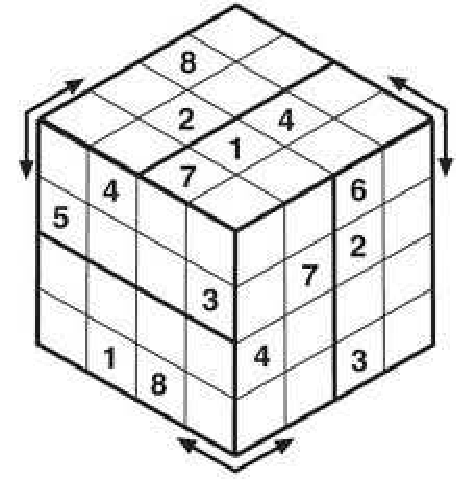
\includegraphics[width=0.3\textwidth]{images}
 \caption{这是一个图片测试例子(中)}
 \label{fig:amss1}
\end{figure}

该页是专门用来测试插入图片的方法,这个方法有很多种,需要自己花点时间来研究学习下,就像表格一样,
下面这只是一个简单的例子。好了,结束。

\subsection{图形位于页面上}
该页是专门用来测试插入图片的方法,这个方法有很多种,需要自己花点时间来研究学习下,就像表格一样,
下面这只是一个简单的例子。好了,结束。该页是专门用来测试插入图片的方法,这个方法有很多种,需要自己花点时间来研究学习下,就像表格一样,
下面这只是一个简单的例子。好了,结束。

\begin{figure}[t]
 \centering
 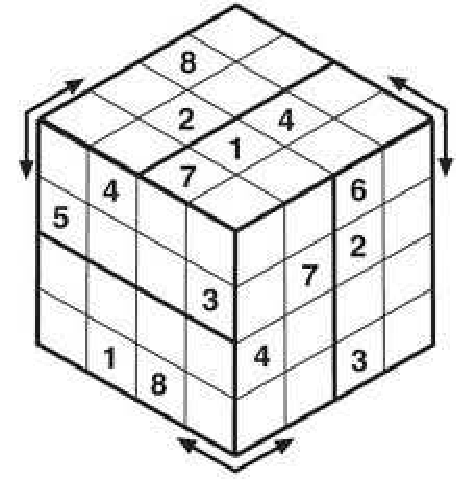
\includegraphics[width=0.3\textwidth]{images}
 \caption{这是一个图片测试例子(上)}
 \label{fig:amss2}
\end{figure}

该页是专门用来测试插入图片的方法,这个方法有很多种,需要自己花点时间来研究学习下,就像表格一样,
下面这只是一个简单的例子。该页是专门用来测试插入图片的方法,这个方法有很多种,需要自己花点时间
来研究学习下,就像表格一样,下面这只是一个简单的例子。该页是专门用来测试插入图片的方法,这个方法
有很多种,需要自己花点时间来研究学习下,就像表格一样,下面这只是一个简单的例子。

\subsection{图形位于页面下}
该页是专门用来测试插入图片的方法,这个方法有很多种,需要自己花点时间来研究学习下,就像表格一样,
下面这只是一个简单的例子。

\begin{figure}[b]
 \centering
 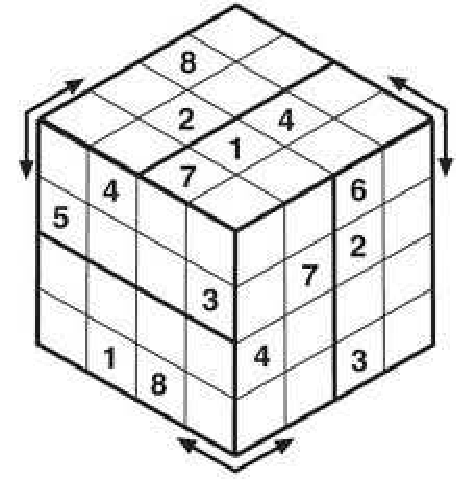
\includegraphics[width=0.3\textwidth]{images}
 \caption{这是一个图片测试例子(下)}
 \label{fig:amss3}
\end{figure}


该页是专门用来测试插入图片的方法,这个方法有很多种,需要自己花点时间来研究学习下,就像表格一样,
下面这只是一个简单的例子。该页是专门用来测试插入图片的方法,这个方法有很多种,需要自己花点时间
来研究学习下,就像表格一样,下面这只是一个简单的例子。

该页是专门用来测试插入图片的方法,这个方法
有很多种,需要自己花点时间来研究学习下,就像表格一样,下面这只是一个简单的例子。该页是专门用来测
试插入图片的方法,这个方法有很多种,需要自己花点时间来研究学习下,就像表格一样,
下面这只是一个简单的例子。

该页是专门用来测试插入图片的方法,这个方法有很多种,需要自己花点时间来研究学习下,就像表格一样,
下面这只是一个简单的例子。该页是专门用来测试插入图片的方法,这个方法有很多种,需要自己花点时间
来研究学习下,就像表格一样,下面这只是一个简单的例子。

该页是专门用来测试插入图片的方法,这个方法
有很多种,需要自己花点时间来研究学习下,就像表格一样,下面这只是一个简单的例子。该页是专门用来测
试插入图片的方法,这个方法有很多种,需要自己花点时间来研究学习下,就像表格一样,
下面这只是一个简单的例子。

该页是专门用来测试插入图片的方法,这个方法有很多种,需要自己花点时间来研究学习下,就像表格一样,
下面这只是一个简单的例子。该页是专门用来测试插入图片的方法,这个方法有很多种,需要自己花点时间
来研究学习下,就像表格一样,下面这只是一个简单的例子。该页是专门用来测试插入图片的方法,这个方法
有很多种,需要自己花点时间来研究学习下,就像表格一样,下面这只是一个简单的例子。该页是专门用来测
试插入图片的方法,这个方法有很多种,需要自己花点时间来研究学习下,就像表格一样,
下面这只是一个简单的例子。


    
\chapter{总结与展望}
\label{chap:con}

\subsection{总结}

\subsection{进一步工作}


    \appendix
    
\chapter[本科生毕业设计论文撰写规范]{西安电子科技大学本科生毕业设计论文撰写规范}
\label{chap:requires}
\section{毕业设计(论文)的总体要求}
撰写论文应简明扼要,一般不少于15000字(外语专业可适当减少,但不得少于10000单词,且须全部用外语书写)。

\section{毕业设计(论文)的编写格式}
每一章、节的格式和版面要求整齐划一、层次清楚。其中:
\begin{itemize}
  \item 论文用纸:统一用A4纸,与论文封皮,任务书,工作计划,成绩考核表一致。
  \item 章的标题:如:"摘要"、"目录"、"第一章"、"附录"等,黑体,三号,居中排列。
  \item 节的标题:如:"2.1  认证方案"、"9.5  小结"等,宋体,四号,居中排列。
  \item 正文:中文为宋体,英文为"Times News Roman",小四号。正文中的图名和表名,宋体,五号。
  \item 页眉:宋体五号,居中排列。左面页眉为论文题目,右面页眉为章次和章标题。页眉底划线的宽度为0.75磅。
  \item 页码:宋体小五号,排在页眉行的最外侧,不加任何修饰。
\end{itemize}

\section{毕业设计(论文)的前置部分}
毕业设计(论文)的前置部分包括封面、中英文摘要、目录等。
\subsection{封面及打印格式}
\begin{itemize}
  \item 学号:按照学校的统一编号,在右上角正确打印自己的学号,宋体,小四号,加粗。
  \item 题目:题目应和任务书的题目一致,黑体,三号。
  \item 学院、专业、班级、学生姓名和导师姓名职称等内容,宋体,小三号,居中排列。
\end{itemize}

\subsection{中英文摘要及关键词}
摘要是关于论文的内容不加注释和评论的简短陈述,具有独立性和自含性。它主要是
简要说明研究工作的目的、方法、结果和结论,重点说明本论文的成果和新见解。关键词
是为了文献标引工作从论文中选取出来用以表示全文主题内容信息的术语。
\begin{enumerate}
  \item 中文摘要,宋体小四号,一般为300字;英文摘要,"Times News Roman"字
体,小四号,一般为300个实词。摘要中不宜出现公式、非公用的符号、术语等。
  \item 每篇论文选取3 \~{} 5个关键词,中文为黑体小四号,英文为"Times News Roman"字体加粗,小四号。关键词排列在摘要的左下方一行,起始格式为:"\textbf{关键词}:
      "和"\textbf{Keyword:}"。具体的各个关键词以均匀间隔排列,之间不加任何分隔符号。
\end{enumerate}

\section{目录}
按照论文的章、节、附录等前后顺序,编写序号、名称和页码。目录页排在中英文摘要之后,主体部分必
须另页右面开始,全文以右页为单页页码。

\section{毕业设计(论文)的主体部分}
毕业设计(论文)的主体部分包括引言(绪论)、正文、结论、结束语、致谢、参考文献。
\subsection{绪论}
作为论文的开端,简要说明作者所做工作的目的、范围、国内外进展情况、前人研究成果、
本人的设想、研究方法等。
\subsection{正文} 为毕业设计(论文)的核心部分,包括理论分析、数据资料、实验方法、结果、本人的论点和结
论等内容,还要附有各种有关的图表、照片、公式等。要求理论正确、逻辑清楚、层次分明、文字流畅、数据真实可
靠,公式推导和计算结果无误,图表绘制要少而精。
\begin{description}
  \item[图] 包括曲线图、示意图、流程图、框图等。图序号一律用阿拉伯数字分章依序编码,如:图1.3、图2.11。每一图应有简短确切的
      图名,连同图序号置于图的正下方。图中坐标上标注的符号和缩略词必须与正文中一致。
  \item[表] 包括分类项目和数据,一般要求分类项目由左至右横排,数据从上到下竖列。分类项目横排中必须标明符号或单位,竖列的数据栏中不宜出现"同上" 、"同左"等类似词语,一律填写具体的数字或文字。表序号一律用阿拉伯数字分章依序编码,如:表2.5、表10.3。每一表应有简短确切的题名,
      连同表序号置于表的正上方。
  \item[公式] 正文中的公式、算式、方程式等必须编排序号,序号一律用阿拉伯数字分章依序编码,如:式(3-32)、式(6-21)。对于较长的公式,另行居中横排,只可在符号处(如:+、-、*、/、$<$、 $>$等)转行。公式序号标注于该式所在行(当有续行时,应标注于最后 一行)的最右边。连续性的公式在"="处排列整齐。大于999的整数或多于三位的小数,一律用半个阿拉伯数字符的小间隔分开;小于1的数应将0置于小数点之前。
  \item[计量单位] 单位名称和符号的书写方式一律采用国际通用符号。
\end{description}

\subsection{结论}
是对主体的最终结论,应准确、完整、精炼。阐述作者创造性工作在本研究领域的地位和作用,对存在的问题和不足应给予客观的说明,也可提出进一步的设想。

\subsection{致谢}
对协助完成论文研究工作的单位和个人表示感谢。

\subsection{参考文献}
在学位论文中引用参考文献时,引出处右上角用方括号标注阿拉伯数字编排的序号(必须与参考文献一致)。参考文献的排列格
式分为:
\begin{description}
  \item[专著类的文献] [序号]  作者 . 专著名称.  版本. 出版地:出版者,出版年. 参考的页码。
  \item[期刊类的文献] 作者 . 文献名. 期刊名称.  年 , 月,  卷(期). 页码。
\end{description}
其中作者采用姓在前、名在后的形式。当作者超过三个时,只著录前三个人,其后
加"等"字即可。

\section{毕业设计(论文)的附录部分}
附录是作为学位论文主体的补充,包括下列内容:
\begin{enumerate}
  \item 正文中过于冗长的公式推导;
  \item 为读者阅读方便所需要的辅助性的数学工作或带有重复性的图表;
  \item 由于过分冗长而不宜在正文中出现的计算机程序清单;
  \item 对于一般读者并非必要阅读,但对本专业同行有参考价值的资料。
  \item 附录编于正文后,与正文连续编页码,每一附录均另页起。
  \item 附录依次用大写正体A,B,C……编序号,黑体,三号。如:附录A。
  \item 附录中的图、表、式、参考文献等与正文分开,用阿拉伯数字另行编序号,注意在数码前冠以附录的
      序码。如:图A1;表B2;式(C-3);文献[D5]。
\end{enumerate}
\section{毕业设计(论文)的打印规格}
论文正文页面和版面的设置规格:论文正文双面打印,为了便于装订、复制,要求每页纸的四周留有足够的空白边缘。以WORD97为例:

页面设置数据为:上3厘米、下2厘米、内侧3厘米、外侧2厘米;装订线 -- 1厘米;页眉  - 2厘米;  页脚 - 1厘米。

版面设置数据为:文字的行间距 - 1. 5倍 ;  公式的行间距 - 1. 5倍字符间距 - 标准;页码数据-对称页边距。

\section{毕业设计(论文)的装订说明}
毕业设计(论文)要求以A4纸的标准,按照下列顺序装订。外文资料翻译原文及译文另册装订,格式参照论文对应内容格式要求。

\begin{enumerate}
  \item 封面
  \item 任务书
  \item 工作计划
  \item 中期检查表
  \item 成绩考核登记表
  \item 中、外论文摘要
  \item 目录
  \item 引言
  \item 论文
  \item 结论
  \item 结束语
  \item 参考文献
  \item 附录
\end{enumerate}












%%----------------- 附件部分 ----------------- %%
    \backmatter
    
\begin{thanks}

毕业论文暂告收尾,这也意味着我在西安电子科技大学的四年的学习生活既将结束。
回首既往,自己一生最宝贵的时光能于这样的校园之中,能在众多学富五车、才华
横溢的老师们的熏陶下度过,实是荣幸之极。在这四年的时间里,我在学习上和思
想上都受益非浅。这除了自身努力外,与各位老师、同学和朋友的关心、支持和鼓
励是分不开的论文的写作是枯燥艰辛而又富有挑战的。

数学是理论界一直探讨的热门话题,老师的谆谆诱导、同学的出谋划策及家长的支持
鼓励,是我坚持完成论文的动力源泉。在此,我特别要感谢我的导师xxx老师。从论文
的选题、文献的采集、框架的设计、结构的布局到最终的论文定稿,从内容到格式,
从标题到标点,她都费尽心血。没有xxx老师的辛勤栽培、孜孜教诲,就没有我论文
的顺利完成。

感谢数学系的各位同学,与他们的交流使我受益颇多。最后要感谢我的家人以及我的
朋友们对我的理解、支持、鼓励和帮助,正是因为有了他们,我所做的一切才更有意
义;也正是因为有了他们,我才有了追求进步的勇气和信心。

时间的仓促及自身专业水平的不足,整篇论文肯定存在尚未发现的缺点和错误。
恳请阅读此篇论文的老师、同学,多予指正,不胜感激!
......

\vskip 18pt

谨把本文献给我最敬爱的父母亲以及所有关心我的人!

\end{thanks}

    
\fontsize{10.5pt}{10.5pt}\selectfont
\begin{thebibliography}{10}

\bibitem{site:ctex}
 http://www.ctex.org


\bibitem{lshort-cn}
\CTeX{}~翻译小组.
\newblock {lshort~中文版~}.
\newblock (2003)


\bibitem{deng:01a}
{邓建松,~彭冉冉,~陈长松}.
\newblock {\LaTeXe{}~科技排版指南}.
\newblock 科学出版社,~书号:~7-03-009239-2/TP.1516, 北京, (2001).

\bibitem{wang:00a}
王磊.
\newblock {\LaTeXe{}~插图指南}.
\newblock (2000).

\bibitem{zhang:03a}
张林波.
\newblock {于新版~CCT~的说明}.
\newblock (2003).

\bibitem{knuth86e}
Donald~E, Knuth.
\newblock {Computer Modern Typefaces}, volume~E of {Computers and
  Typesetting}.
\newblock Addison-Wesley, Reading, Massachusetts, (1986).

\bibitem{knuth86d}
Donald~E. Knuth.
\newblock {{METAFONT}: The Program}, volume~D of {Computers and
  Typesetting}.
\newblock Addison-Wesley, Reading, Massachusetts, (1986).

\bibitem{knuth86c}
Donald~E. Knuth.
\newblock {The {METAFONT}book}, volume~C of {Computers and
  Typesetting}.
\newblock Addison-Wesley, Reading, Massachusetts, (1986).

\bibitem{knuth86b}
Donald~E. Knuth.
\newblock {{\TeX}: The Program}, volume~B of { Computers and
  Typesetting}.
\newblock Addison-Wesley, Reading, Massachusetts, (1986).

\bibitem{knuth86a}
Donald~E. Knuth.
\newblock {The {TeX}book}, volume~A of {Computers and Typesetting}.
\newblock Addison-Wesley, Reading, Massachusetts, (1986).

\bibitem{lamport85a}
Leslie Lamport.
\newblock {{\LaTeX} --- A Document Preparation System: User's Guide and
  Reference Manual}.
\newblock Addison-Wesley, Reading, Massachusetts, 2nd edition, (1985).

\end{thebibliography}


\end{document}



